\chapter{Challenge II}
\section{Outline}
\begin{enumerate}
   \item Each subject manages a list with its own capabilities
   
   \item The operation field of a capability is encrypted with a key private to the security kernel SK
   
   \item To request operation Op on object O, a subject S sends to SK a message with S, O, Op and the encrypted capability
   
   \item SK decrypts the capability and, if it enables Op on O, it asks O to create a channel with S to execute OP
   
   \item O destroys the channel when Op ends
\end{enumerate}

\begin{figure}[htbp]
   \centering
   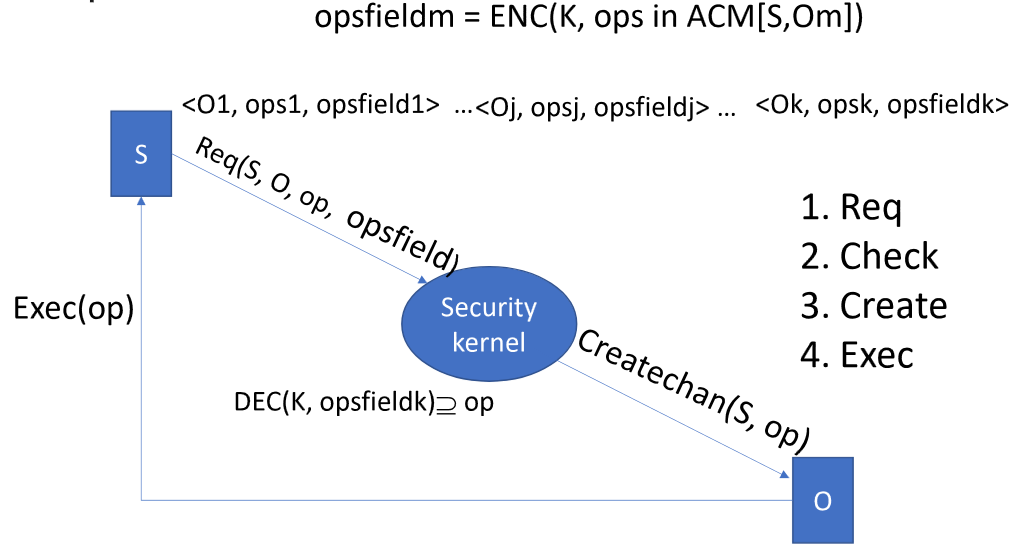
\includegraphics{images/challenge_2.png}
   \caption{Protocol schema}
   \label{fig:challenge_2}
\end{figure}

\subsection{Request}
Discover vulnerabilities in the proposed protocol or in the overall system under the assumption that there are no vulnerabilities in the encryption algorithm,
i.e. K cannnot be discovered because of  mathematical vulnerabilities.

\section{Proposed Solutions}
\subsection{Vulnerability 1}
